% Dotter User Manual
% Author: Gemma Barson
%
% Run the following command twice to create a pdf of this manual
% (two runs are necessary to make sure all of the cross-references
% are up to date):
%
%    pdflatex Dotter_manual.tex
%
% This file was converted to LaTeX by Writer2LaTeX ver. 1.0.2
% see http://writer2latex.sourceforge.net for more info
\documentclass[letterpaper]{article}
\usepackage[latin1]{inputenc}
\usepackage[T1]{fontenc}
\usepackage[english]{babel}
\usepackage{amsmath}
\usepackage{amssymb,amsfonts,textcomp}
\usepackage{color}
\usepackage{array}
\usepackage{supertabular}
\usepackage{hhline}
\usepackage{hyperref}
\usepackage{titlesec}
\hypersetup{pdftex, colorlinks=true, linkcolor=blue, citecolor=blue, filecolor=blue, urlcolor=blue, pdftitle=Dotter User Manual, pdfauthor=Gemma Barson, pdfsubject=, pdfkeywords=}
\usepackage[pdftex]{graphicx}
% Paragraph styles
\setlength{\parindent}{0pt}
% Text styles
\newcommand\textstyleInternetlink[1]{\textcolor{blue}{#1}}
\newcommand\textstyleSourceText[1]{\texttt{#1}}
\newcommand\textstyleFootnoteSymbol[1]{\textsuperscript{#1}}
\definecolor{darkblue}{rgb}{0.2,0.3,0.5}
\definecolor{lightblue}{rgb}{0.3,0.5,0.8}
%\DeclareFixedFont{\sectionfont}{T1}{phv}{bx}{n}{16pt}
%\DeclareFixedFont{\subsectionfont}{T1}{phv}{bx}{n}{14pt}
%\DeclareFixedFont{\subsubsectionfont}{T1}{phv}{bx}{n}{12pt}
\titleformat{\section} {\normalfont\LARGE\bf\color{darkblue}}{\thesection}{1em}{}
\titleformat{\subsection} {\normalfont\large\bf\color{lightblue}}{\thesubsection}{1em}{}
\titleformat{\subsubsection} {\normalfont\normalsize\bf\color{lightblue}}{\thesubsubsection}{1em}{}
% Outline numbering
\setcounter{secnumdepth}{0}
\makeatletter
\newcommand\arraybslash{\let\\\@arraycr}
\makeatother
% List styles
\newcommand\liststyleLi{%
\renewcommand\labelitemi{{\textbullet}}
\renewcommand\labelitemii{{\textbullet}}
\renewcommand\labelitemiii{{\textbullet}}
\renewcommand\labelitemiv{{\textbullet}}
}
\newcommand\liststyleLii{%
\renewcommand\labelitemi{{\textbullet}}
\renewcommand\labelitemii{{\textbullet}}
\renewcommand\labelitemiii{{\textbullet}}
\renewcommand\labelitemiv{{\textbullet}}
}
\newcommand\liststyleLiii{%
\renewcommand\labelitemi{{\textbullet}}
\renewcommand\labelitemii{{\textbullet}}
\renewcommand\labelitemiii{{\textbullet}}
\renewcommand\labelitemiv{{\textbullet}}
}
\newcommand\liststyleWWviiiNumxxxvi{%
\renewcommand\labelitemi{{\textbullet}}
\renewcommand\labelitemii{o}
\renewcommand\labelitemiii{[F0A7?]}
\renewcommand\labelitemiv{[F0B7?]}
}
\newcommand\liststyleLiv{%
\renewcommand\labelitemi{{\textbullet}}
\renewcommand\labelitemii{${\circ}$}
\renewcommand\labelitemiii{${\blacksquare}$}
\renewcommand\labelitemiv{{\textbullet}}
}
\newcommand\liststyleWWviiiNumxxxi{%
\renewcommand\theenumi{\arabic{enumi}}
\renewcommand\theenumii{\alph{enumii}}
\renewcommand\theenumiii{\roman{enumiii}}
\renewcommand\theenumiv{\arabic{enumiv}}
\renewcommand\labelenumi{\theenumi.}
\renewcommand\labelenumii{\theenumii.}
\renewcommand\labelenumiii{\theenumiii.}
\renewcommand\labelenumiv{\theenumiv.}
}
\newcommand\liststyleWWviiiNumxxxv{%
\renewcommand\labelitemi{{\textbullet}}
\renewcommand\labelitemii{o}
\renewcommand\labelitemiii{[F0A7?]}
\renewcommand\labelitemiv{[F0B7?]}
}
\newcommand\liststyleWWviiiNumxiii{%
\renewcommand\labelitemi{{\textbullet}}
\renewcommand\labelitemii{o}
\renewcommand\labelitemiii{[F0A7?]}
\renewcommand\labelitemiv{[F0B7?]}
}
\newcommand\liststyleWWviiiNumxxvii{%
\renewcommand\labelitemi{{\textbullet}}
\renewcommand\labelitemii{o}
\renewcommand\labelitemiii{[F0A7?]}
\renewcommand\labelitemiv{[F0B7?]}
}
\newcommand\liststyleWWviiiNumxxvi{%
\renewcommand\labelitemi{{\textbullet}}
\renewcommand\labelitemii{o}
\renewcommand\labelitemiii{[F0A7?]}
\renewcommand\labelitemiv{[F0B7?]}
}
\newcommand\liststyleWWviiiNumxvi{%
\renewcommand\labelitemi{{\textbullet}}
\renewcommand\labelitemii{o}
\renewcommand\labelitemiii{[F0A7?]}
\renewcommand\labelitemiv{[F0B7?]}
}
\newcommand\liststyleWWviiiNumxxxvii{%
\renewcommand\labelitemi{{\textbullet}}
\renewcommand\labelitemii{o}
\renewcommand\labelitemiii{[F0A7?]}
\renewcommand\labelitemiv{[F0B7?]}
}
\newcommand\liststyleWWviiiNumxx{%
\renewcommand\labelitemi{{\textbullet}}
\renewcommand\labelitemii{o}
\renewcommand\labelitemiii{[F0A7?]}
\renewcommand\labelitemiv{[F0B7?]}
}
% Page layout (geometry)
\setlength\voffset{-1in}
\setlength\hoffset{-1in}
\setlength\topmargin{2.54cm}
\setlength\oddsidemargin{3.175cm}
\setlength\textheight{21.363003cm}
\setlength\textwidth{15.240001cm}
\setlength\footskip{1.497cm}
\setlength\headheight{0cm}
\setlength\headsep{0cm}
% Footnote rule
\setlength{\skip\footins}{0.119cm}
\renewcommand\footnoterule{\vspace*{-0.018cm}\setlength\leftskip{0pt}\setlength\rightskip{0pt plus 1fil}\noindent\textcolor{black}{\rule{0.25\columnwidth}{0.018cm}}\vspace*{0.101cm}}
% Pages styles
\makeatletter
\newcommand\ps@Standard{
  \renewcommand\@oddhead{}
  \renewcommand\@evenhead{}
  \renewcommand\@oddfoot{\thepage{}}
  \renewcommand\@evenfoot{\@oddfoot}
  \renewcommand\thepage{\arabic{page}}
}
\newcommand\ps@FirstPage{
  \renewcommand\@oddhead{}
  \renewcommand\@evenhead{}
  \renewcommand\@oddfoot{}
  \renewcommand\@evenfoot{}
  \renewcommand\thepage{\arabic{page}}
}
\makeatother
\pagestyle{Standard}
\setlength\tabcolsep{1mm}
\renewcommand\arraystretch{1.3}
% footnotes configuration
\makeatletter
\renewcommand\thefootnote{\arabic{footnote}}
\makeatother
\newcounter{Figure}
\renewcommand\theFigure{\arabic{Figure}}

\title{Dotter User Manual}
\author{Gemma Barson}
\date{2011-01-18}

\begin{document}

\setcounter{page}{1}\pagestyle{Standard}

\thispagestyle{FirstPage}
{\centering\sffamily\bfseries\color[rgb]{0.0,0.27058825,0.5254902}
\Huge\bf{Dotter User Manual}
\par}

\bigskip

{\centering
\large{Written by Gemma Barson}
\par}
{\centering
{\textless}\href{mailto:gb10@sanger.ac.uk}{gb10@sanger.ac.uk}{\textgreater}
\par}

\bigskip

{\centering
\large{Wellcome Trust Sanger Institute}
\par}
{\centering
18 January 2011
\par}



\clearpage{\color[rgb]{0.0,0.27058825,0.5254902}\section[Revision History]{Revision History}}

\begin{center}
\tablehead{}
\begin{supertabular}{|m{8.073cm}|m{3.2849998cm}|m{3.282cm}|}
\hline
\bfseries Revision &
\bfseries Date &
\bfseries Author\\\hline
 First revision (Dotter v4.1.5) &
 18/01/11 &
 Gemma Barson\\\hline
 Updated for Dotter v4.1.9 &
 10/02/11 &
 Gemma Barson\\\hline
 Updated for Dotter v4.1.13 &
 25/03/11 &
 Gemma Barson\\\hline
 Updated for Dotter v4.1.14 &
 04/04/11 &
 Gemma Barson\\\hline
 Updated for Dotter v4.7 &
 02/12/11 &
 Gemma Barson\\\hline
Updated for Dotter v4.27 &
 17/04/14 &
 Gemma Barson\\\hline
~
 &
~
 &
~
\\\hline
~
 &
~
 &
~
\\\hline
~
 &
~
 &
~
\\\hline
~
 &
~
 &
~
\\\hline
~
 &
~
 &
~
\\\hline
~
 &
~
 &
~
\\\hline
~
 &
~
 &
~
\\\hline
~
 &
~
 &
~
\\\hline
~
 &
~
 &
~
\\\hline
~
 &
~
 &
~
\\\hline
\end{supertabular}
\end{center}



\setcounter{tocdepth}{10}
\renewcommand\contentsname{Contents}

\clearpage
\tableofcontents

\clearpage{\color[rgb]{0.0,0.27058825,0.5254902}\section[Introduction]{Introduction}}
{This manual explains how to configure, run and
use Dotter. Dotter is a graphical
dot-plot program for detailed comparison of two sequences.
Every residue in one sequence is compared to every residue
in the other sequence. \ The first sequence runs along the x-axis and
the second sequence along the y-axis. \ In regions where the two
sequences are similar to each other, a row of high scores will run
diagonally across the dot matrix.}

\bigskip

{Pairwise scores are averaged over a sliding window to make the
score matrix more intelligible. The averaged score matrix
forms a three-dimensional landscape, with the two sequences in two
dimensions and the height of the peaks in the third. This landscape is
projected onto two dimensions using a grey-scale image - the darker
grey of a peak, the higher the score is.}

\bigskip

{The contrast and threshold of the grey-scale image can be adjusted, and
a tool is provided to examine the sequence alignment that the
grey-scale image represents.}

\bigskip

Dotter is maintained by the Wellcome Trust
Sanger Institute and is available as part of the SeqTools package.
\ The software can be downloaded from the Sanger
Institute{\textquoteright}s website:

\href{http://www.sanger.ac.uk/resources/software/seqtools/}
{\textstyleInternetlink{http://www.sanger.ac.uk/resources/software/seqtools}}

{\color[rgb]{0.0,0.27058825,0.5254902}\section[Getting Started]{Getting Started}}
{\color[rgb]{0.30980393,0.5058824,0.7411765}\subsection[Running Dotter]{Running Dotter}}

As a minimum, Dotter takes the following required arguments:

\begin{quote}
\begin{verbatim}
dotter <horizontal_sequence> <vertical_sequence>
\end{verbatim}
\end{quote}

where \texttt{{\textless}horizontal\_sequence{\textgreater}} and
\texttt{{\textless}vertical\_sequence{\textgreater}} are the path names of FASTA
files containing the two input sequences.
Dotter will assume that the sequences both start at coordinate 1 unless
you use the {}-q and {}-s arguments to set an offset for the query
(horizontal) and subject (vertical) sequences respectively.

\bigskip

Run {\textquoteleft}dotter{\textquoteleft} without any arguments to see
further usage information.

{\color[rgb]{0.30980393,0.5058824,0.7411765}\subsubsection[Sequence versus itself]{Sequence versus itself}}
{Dotter can be run on a sequence versus itself. \ This can be useful to
analyse internal repeats. \ You can also look for overlaps between many
sequences by making a dot-plot of all of the sequences versus
themselves. \ To run Dotter on many sequences at once, concatenate the
FASTA files for all of the sequences and then run Dotter on the
concatenated sequence file against itself.}

\bigskip

{If you{\textquotesingle}re comparing a sequence against itself,
you{\textquotesingle}ll notice that the main diagonal scores maximally,
since it{\textquotesingle}s the 100\% perfect self-match.
\ Partitioning break-lines will appear between the sequences if there
were multiple sequences in the input file.}

\begin{figure}
 \centering
 \color[rgb]{0.30980393,0.5058824,0.7411765}
 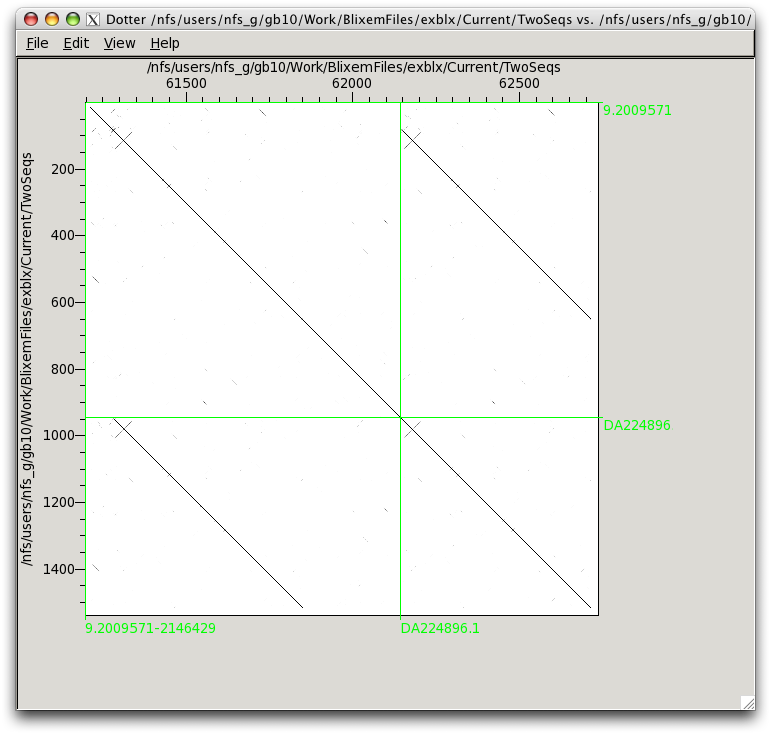
\includegraphics[width=15.24cm,height=14.508cm]{img_window_dotter_self.png}
 \caption{Multiple sequences vs themselves}
\end{figure}

\bigskip

{\color[rgb]{0.30980393,0.5058824,0.7411765}\subsection[Input files]{Input files}}
{The sequence input files are in FASTA format. \ Comparisons are allowed
between two nucleotide sequences, two protein sequences, or one
nucleotide and one protein sequence -- note that when comparing a
nucleotide and a protein sequence, the nucleotide sequence must be
passed first (i.e. as the horizontal sequence).}

\bigskip

{Additional features can be passed to Dotter in a GFF file using the {}-f
argument. \ Relevant features include alignments, which can be viewed
using Dotter{\textquotesingle}s HSP mode, and transcripts, which are
shown at the bottom of the Dotter window.}

\bigskip

{\color[rgb]{0.30980393,0.5058824,0.7411765}\subsubsection[FASTA file]{FASTA file}}
{A FASTA file has a header line that starts with
{\textquoteleft}{\textgreater}{\textquoteright} and contains the
sequence name. \ The next line contains the start of the sequence data.
\ The sequence data can be on a single line or separated by newlines;
it is usually separated by newlines every 50 characters to aid
readability.}

\bigskip

\begin{quote}
\begin{verbatim}
>chr4-04
tcttgtttctgtaggagaggccatctccatcagctataaccaaaaaaaaa
acaaaaaactcctctttttgacaagtttgtaaagcctgtccatctgggtc
tataataatcctccaggccctatgccactcctctttattcagccagttca
...
\end{verbatim}
\end{quote}

{\color[rgb]{0.30980393,0.5058824,0.7411765}\subsubsection[GFF file]{GFF file}}
{Dotter uses the GFF version 3 file format. \ In this section we give a
very brief description of this file format; see
\url{http://www.sequenceontology.org/gff3.shtml} for a full
description.}

\bigskip

{The GFF file should start with the following two comment lines.
\ (Additional comments can be included but may be ignored.)

\bigskip

\begin{quote}
\begin{verbatim}
##gff-version 3
##sequence-region chr4-04 44144 154265
\end{verbatim}
\end{quote}
Each subsequent line defines a feature. \ A feature line must have the
following 8 tab-separated columns:
\begin{quote}
\begin{verbatim}
reference_sequence_name source type start end score strand phase
\end{verbatim}
\end{quote}
An optional 9\textsuperscript{th} column defines any tags (separated by
semi-colons). \ Dotter supports the following GFF tags. \ (Additional
tags can be supplied but may be ignored.)

\begin{center}
\begin{supertabular}{p{2.802cm}p{10.704cm}}
\textbf{Target } & (required for alignments) \\
\textbf{Gap} & (required for gapped alignments) \\
\textbf{ID } & (required for parent features) \\
\textbf{Name } & (required for transcripts and SNPs) \\
\textbf{Parent } & (required for child features) \\
\end{supertabular}
\end{center}
}

{\color[rgb]{0.30980393,0.5058824,0.7411765}\subsubsection{Transcripts}}
{Note that exons should have a Parent transcript defined, and the Name
tag should be set in the parent rather than the child exons. \ Note
that Dotter \textit{will} recognise exons that do not have a Parent tag
if they have a Name tag instead, but they may not get grouped correctly
with other exons from the same transcript.}

\bigskip

{Typically, one defines the parent transcript, the exons, and the CDS
regions; Dotter will then calculate the missing components (in this
case, the UTR regions and the introns). \ Dotter will recognise other
combinations of inputs, and will always calculate the missing
components as long as enough information is provided. }

\bigskip
{\color[rgb]{0.30980393,0.5058824,0.7411765}\subsubsection{Sample GFF file}}
{A sample GFF file may look like this ({\textquoteleft}{\dots}{\textquoteleft} denotes that text has been
omitted).}

\bigskip

\begin{quote}
\begin{verbatim}
##gff-version 3
##sequence-region chr4-04 44144 154265
chr4-04 EST_Human nucleotide_match 79195 79311 95.000000 - . Target=DA692754.1 \
287 403 +;percentID=90.6;sequence=GATCTGGC...
chr4-04 EST_Human nucleotide_match 79195 79323 121.000000 + . Target=AI095103.1 \
326 454 +;percentID=96.9;sequence=TTTAAATT...
chr4-04 ensembl_variation deletion 80798 80799 . + . Name=rs60725655;url=http%3A\
%2F%2Fwww.ensembl.org%2FHomo_sapiens%2FVariation%2FSummary%3Fv%3Drs60725655;vari\
ant_sequence=AA-;
chr4-04 Augustus mRNA 119534 119941 . - . ID=transcript21;Name=AUGUSTUS00000051712
chr4-04 Augustus exon 119534 119941 . - . Parent=transcript21
chr4-04 Augustus CDS 119534 119941 . - 0 Parent=transcript21
\end{verbatim}
\end{quote}

{\color[rgb]{0.0,0.27058825,0.5254902}\section[The Dotter Windows]{The Dotter Windows}}
{\color[rgb]{0.30980393,0.5058824,0.7411765}\subsection[The dot{}-plot window]{The dot-plot window}}
{The main Dotter window contains the dot-matrix plot. \ It also shows any
exons for the sequences along the bottom of the window (for the
horizontal sequence; or along the right-hand-side for the vertical
sequence).}

\begin{figure}
 \centering
 \color[rgb]{0.30980393,0.5058824,0.7411765}
  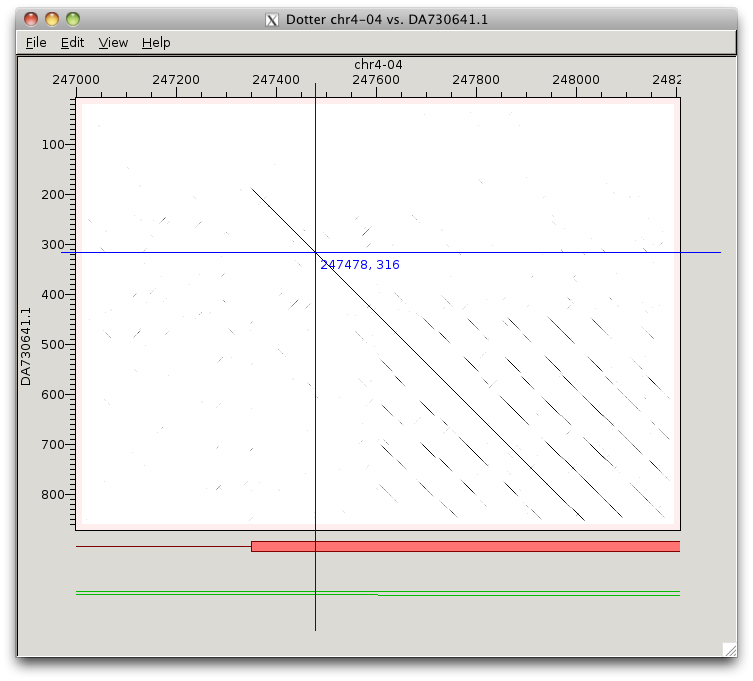
\includegraphics[width=14.88cm,height=13.457cm]{img_window_main.png}
 \caption{The main window}
\end{figure}

\bigskip

{Note that the narrow red-shaded border around the edge of the plot
indicates the region where the dot-plot cannot be calculated due to the
sliding window averaging method that is used to calculate the scores. }

\bigskip
{\color[rgb]{0.30980393,0.5058824,0.7411765}\subsubsection[Cross{}-hair]{Cross-hair}}
{The blue cross-hair shows the coordinates at a particular position. \ It
can be moved by clicking/dragging with the left mouse button, or by
using the following keyboard shortcuts:}

\begin{center}
\tablehead{}
\begin{supertabular}{p{2.802cm}p{10.704cm}}
{\bfseries Left-arrow}

\bfseries Right-arrow &
 Move one dot left/right along the horizontal
sequence.\\
{\bfseries Shift-Left}

\bfseries Shift-Right &
 The same as Left/Right, but for protein
sequences this moves by a single nucleotide coordinate rather than a
whole dot/amino-acid.\\
{\bfseries Up-arrow}

\bfseries Down-arrow &
 Move one dot up/down along the vertical
sequence.\\
{\bfseries Shift-Up}

\bfseries Shift-Down &
 The same as Up/Down, but for protein sequences
this moves by a single nucleotide coordinate rather than a whole
dot/amino-acid.\\
{\bfseries ,}

\bfseries . &
 Move diagonally up-left or down-right. \ Useful
for moving along an alignment.\\
{\bfseries {\textless}}

\bfseries {\textgreater} &
 Move diagonally up-left or down-right but, for
protein sequences, move by a single nucleotide coordinate rather than a
whole amino-acid.\\
{\bfseries [}

\bfseries ] &
 Move diagonally down-left or up-right. \ Useful
for moving along an alignment.\\
{\bfseries \{}

\bfseries \} &
 Move diagonally down-left or up-right but, for
protein sequences, move by a single nucleotide coordinate rather than a
whole amino-acid.\\
\end{supertabular}
\end{center}

{\color[rgb]{0.30980393,0.5058824,0.7411765}\subsubsection[Zoom in with a child Dotter]{Zoom in with a child Dotter}}
{You can open a new child Dotter on a particular region from the current
Dotter window. \ Middle-click and drag the mouse to select the region
to open the new Dotter on.}

\bigskip

{\color[rgb]{0.30980393,0.5058824,0.7411765}\subsection[The alignment tool]{The alignment tool}}
{The alignment tool shows the portions of the two sequences at the
current cross-hair position. \ The sequences will move to remain
centred on the cross-hair coordinates when the cross-hair is moved.
\ The same shortcut keys for moving the cross-hair can be used in this
window.}

\bigskip

{Aligning matches are highlighted and colour-coded according to whether
they are an exact or conserved match (cyan for exact, violet for
conserved).}

\bigskip

{In nucleotide-{\textgreater}nucleotide mode, both strands of the
horizontal sequence are shown in the alignment tool. \ In
nucleotide-{\textgreater}protein mode, all three reading frames of the
horizontal sequence are shown, and the best match out of the three
frames determines the highlight colour for the bases in the vertical
sequence.}

\bigskip

{If closed or hidden, the alignment tool can be shown with the
{\textquotesingle}Ctrl-A{\textquotesingle} shortcut or by selecting the
{\textquotesingle}Alignment tool{\textquotesingle} option under the
{\textquotesingle}View{\textquotesingle} menu.}

\begin{figure}
 \centering
 \color[rgb]{0.30980393,0.5058824,0.7411765}
 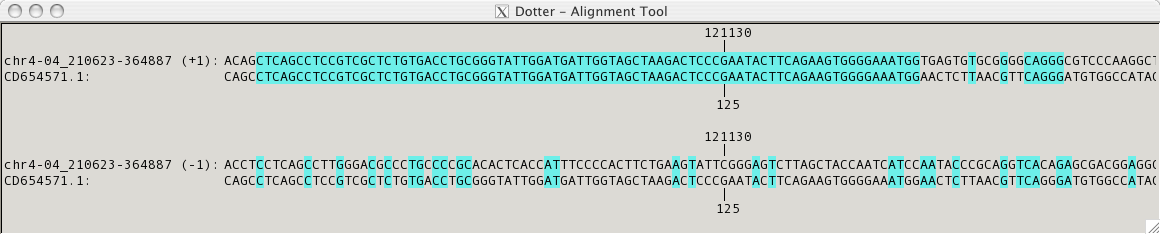
\includegraphics[width=15.24cm,height=3.074cm]{img_window_nucleotide.png}
 \caption{Alignment tool - nucleotide-{\textgreater}nucleotide mode}
\end{figure}

\begin{figure}
 \centering
 \color[rgb]{0.30980393,0.5058824,0.7411765}
 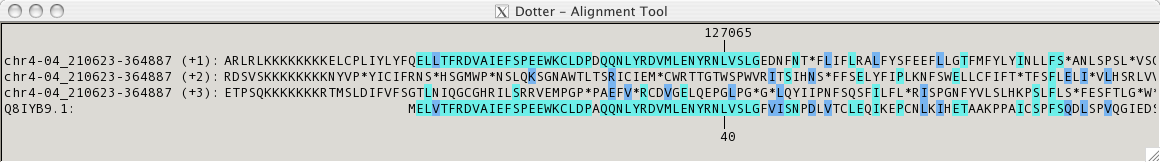
\includegraphics[width=15.24cm,height=2.127cm]{img_window_protein.png}
 \caption{Alignment tool - nucleotide-{\textgreater}protein mode}
\end{figure}

\bigskip

{\color[rgb]{0.30980393,0.5058824,0.7411765}\subsubsection[Alignment tool menu ]{Alignment tool menu }}
{Right-clicking in the alignment tool brings up a context menu with the
following options:}

\begin{center}
\tablehead{}
\begin{supertabular}{p{3.853cm}p{9.653cm}}
\bfseries Copy horizontal coord &
 Copy the current horizontal-sequence coordinate
to the clipboard\\
\bfseries Copy vertical coord &
 Copy the current vertical-sequence coordinate
to the clipboard\\
\bfseries Close tool &
 Close the alignment tool window (it can be
re-opened with Ctrl-A)\\
\bfseries Print &
 Print the alignment tool window\\
\bfseries Set alignment Left &
 Control how long a portion of the sequences
should be shown in the alignment tool.\\
\end{supertabular}
\end{center}

\begin{figure}
 \centering
 \color[rgb]{0.30980393,0.5058824,0.7411765}
 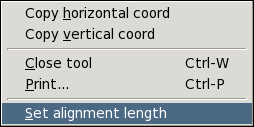
\includegraphics[width=6.853cm,height=3.12cm]{img_menu_alignment_tool.png}
 \caption{Alignment tool menu}
\end{figure}

{\color[rgb]{0.30980393,0.5058824,0.7411765}\subsubsection[Alignment tool shortcuts]{Alignment tool shortcuts}}
{The keyboard shortcuts for moving the cross-hair also apply in the
alignment tool window.}

\bigskip
{\color[rgb]{0.30980393,0.5058824,0.7411765}\subsection[Greyramp tool]{Greyramp tool}}
{This tool controls the threshold and contrast of the the dot-plot image.
\ To improve visualization, little peaks (noise) can be nullified by a
minimum cut-off. \ Similarly, significant peaks above a certain score
can be saturated by a maximum cut-off. }

\bigskip

{Drag the square handle and the arrows to change the threshold and
contrast. \ The {\textquotesingle}Swap{\textquotesingle} button swaps
the positions of the top and bottom arrows, inverting the colours.
\ The {\textquotesingle}Undo{\textquotesingle} button undoes the effect
of the last drag.}

\bigskip

{If closed or hidden, the greyramp tool can be shown with the
{\textquotesingle}Ctrl-G{\textquotesingle} shortcut or by selecting the
{\textquotesingle}Greyramp tool{\textquotesingle} option under the
{\textquotesingle}View{\textquotesingle} menu.}

\begin{figure}
 \centering
 \color[rgb]{0.30980393,0.5058824,0.7411765}
 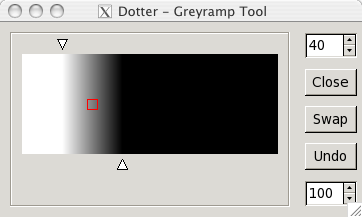
\includegraphics[width=9.287cm,height=5.567cm]{img_window_greyramp.png}
 \caption{Greyramp tool}
\end{figure}

\bigskip

{\color[rgb]{0.0,0.27058825,0.5254902}\section[Main menu]{Main menu}}
{The main menu can be accessed via the menu-bar at the top of the
dot-plot window or by right-clicking in the dot-plot window.}

\bigskip

{Note that menus with a dotted line at the top can be
{\textquotedblleft}torn off{\textquotedblright} by clicking on the
dotted line. \ A torn-off menu will stay visible on top of the Dotter
window and can be repositioned by dragging its header bar. \ Click the
dotted line again to get rid of it. }

\begin{figure}
 \centering
 \color[rgb]{0.30980393,0.5058824,0.7411765}
 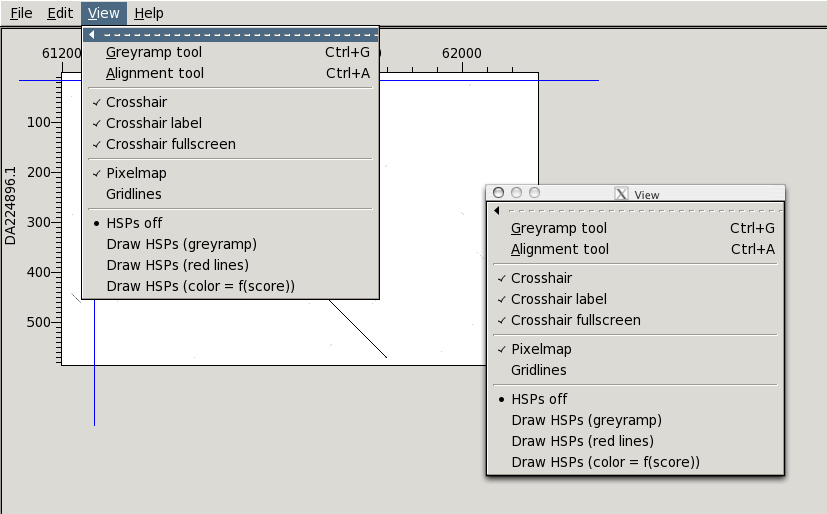
\includegraphics[width=15.24cm,height=9.47cm]{img_menu_tear_off.png}
 \caption{Tear-off menus}
\end{figure}

\bigskip

{\color[rgb]{0.30980393,0.5058824,0.7411765}\subsection[File menu]{File menu}}

\begin{figure}
 \centering
 \color[rgb]{0.30980393,0.5058824,0.7411765}
 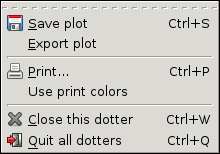
\includegraphics[width=6.69cm,height=4.685cm]{img_menu_file.png}
 \caption{File menu}
\end{figure}

\begin{center}
\tablehead{}
\begin{supertabular}{p{2.135cm}p{11.371cm}}
 \textbf{Save plot}  &
 Save the current dot-plot. \ It can be
re-loaded by calling Dotter from the command line using the -l
argument. \ Note that you will need to call Dotter with the same
portion of each sequence that was originally passed to Dotter in order
for the alignment tool to function correctly when you load the
dot-plot.\\
\bfseries Export plot &
 Export the plot to PDF format. \ Note that
other formats are also available from the Print menu by selecting Print
to File from the print dialog.\\
\bfseries Print &
 Print the current dot-plot.\\
\bfseries Use print colours &
 Change to a colour-scheme that is more suitable
for printing.\\
\bfseries Close &
 Close the current Dotter window. \ Also closes
the associated alignment and greyramp tool, but does not close any
other Dotter windows.\\
\bfseries Quit  &
 Close the current Dotter window and all
associated Dotters as well (including any child or parent Dotters).
\ If you just wish to close the current Dotter, then use the
{\textquotesingle}Close{\textquotesingle} menu option instead.\\
\end{supertabular}
\end{center}

{ \color[rgb]{0.30980393,0.5058824,0.7411765}\subsection[Edit menu]{Edit menu}}

\begin{figure}
 \centering
 \color[rgb]{0.30980393,0.5058824,0.7411765}
 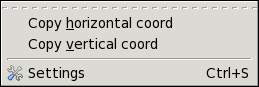
\includegraphics[width=7.638cm,height=2.431cm]{img_menu_edit.png}
 \caption{Edit menu}
\end{figure}

\begin{center}
\tablehead{}
\begin{supertabular}{p{4.000cm}p{9.506cm}}
\bfseries Copy horizontal coord &
 Copy the current horizontal-sequence coordinate
to the clipboard\\
\bfseries Copy vertical coord &
 Copy the current vertical-sequence coordinate
to the clipboard\\
 \textbf{Settings}  &
 Show the
{\textquotesingle}Settings{\textquotesingle} dialog.\\
\end{supertabular}
\end{center}

{ \color[rgb]{0.30980393,0.5058824,0.7411765}\subsection[View menu]{View menu}}

\begin{figure}
 \centering
 \color[rgb]{0.30980393,0.5058824,0.7411765}
 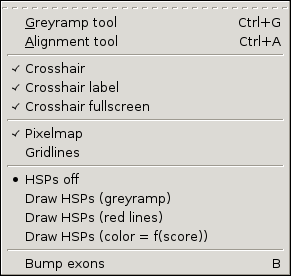
\includegraphics[width=7.303cm,height=7.454cm]{img_menu_view.png}
 \caption{View menu}
\end{figure}

\begin{center}
\tablehead{}
\begin{supertabular}{p{2.649cm}p{10.858cm}}
\bfseries Greyramp tool &
 Show the greyramp tool.\\
\bfseries Alignment tool &
 Show the alignment tool.\\
\bfseries Crosshair &
 Toggle visibility of the cross-hair\\
\bfseries Crosshair label &
 Toggle visibility of the cross-hair label (only
has an effect if the cross-hair is visible).\\
\bfseries Crosshair fullscreen &
 Toggle whether the cross-hair is shown to its
full extents or is clipped to just the dot-plot area.\\
\bfseries Pixelmap &
 Toggle visibility of the grey-scale dot-plot
image.\\
\bfseries Gridlines &
 Toggle visibility of gridlines.\\
\bfseries HSPs off &
 Select this option to turn HSP (High Scoring
Pair) mode off.\\
\bfseries Draw HSPs (greyramp) &
 Select this option to view HSPs in grey-scale
mode. \ In this mode, the HSPs (High Scoring Pairs) are drawn in a
shade of grey that is determined by their score. \ The greyramp tool
can be used to adjust the thresholds and contrast of the HSP image.
\ This mode \textit{replaces} the standard dot-plot image.\\
\bfseries Draw HSPs (red lines) &
 Select this option to view all HSPs as red
lines. \ This mode can be used in conjunction with the standard
dot-plot image: HSPs are drawn over the top.\\
\bfseries Draw HSPs (color=f(score)) &
 Select this option to view HSPs as solid lines,
whose colour depends on their score. \ This mode can be used in
conjunction with the standard dot-plot image: HSPs are drawn over the
top.\\
\bfseries Bump exons &
 Expand the transcript display so that exons do
not overlap.\\
\end{supertabular}
\end{center}

{ \color[rgb]{0.30980393,0.5058824,0.7411765}\subsection[Help menu]{Help menu}}

\begin{figure}
 \centering
 \color[rgb]{0.30980393,0.5058824,0.7411765}
 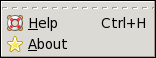
\includegraphics[width=4.68cm,height=1.51cm]{img_menu_help.png}
 \caption{Help menu}
\end{figure}

\begin{center}
\tablehead{}
\begin{supertabular}{p{2.649cm}p{10.858cm}}
\bfseries Help &
 Show the {\textquotesingle}Help{\textquotesingle} dialog.\\
\bfseries About &
 Show the
{\textquotesingle}About{\textquotesingle} dialog.\\
\end{supertabular}
\end{center}

{\color[rgb]{0.0,0.27058825,0.5254902}\section[Settings]{Settings}}

{The settings dialog can be accessed by selecting the
{\textquotesingle}Settings{\textquotesingle} option on the
{\textquotesingle}Edit{\textquotesingle} menu, or by pressing the
{\textquotesingle}Ctrl-S{\textquotesingle} shortcut key.}

\begin{figure}
 \centering
 \color[rgb]{0.30980393,0.5058824,0.7411765}
 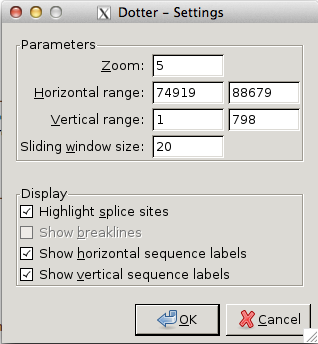
\includegraphics[width=7.953cm]{img_dialog_settings.png}
 \caption{The Settings dialog}
\end{figure}

\bigskip

{\color[rgb]{0.30980393,0.5058824,0.7411765}\subsubsection[Zoom]{Zoom}}
{Specify the zoom factor. \ The factor is an inverse: a zoom factor of 3
will zoom \textit{out} by a factor of 3, i.e. the window will shrink to
1/3 of its full size. \ A zoom factor of 1 will show the window at full
size. \ A factor of less than 1 (e.g. 0.5) can be set in order to zoom
in, but this will result in a stretched dot-plot so is not
recommended.}

\bigskip

{\color[rgb]{0.30980393,0.5058824,0.7411765}\subsubsection[Horizontal range]{Horizontal range}}
{Set the range of the horizontal sequence. \ The maximum range possible
is the range that was originally passed to Dotter -- the range you
enter will be trimmed if you enter out-of-range values.}

\bigskip

{\itshape
Note that this causes the matrix to be recalculated, so if it took a
long time to calculate in the first place, stay away from this menu
item!}

\bigskip

{\color[rgb]{0.30980393,0.5058824,0.7411765}\subsubsection[Vertical range]{Vertical range}}
{Set the range of the vertical sequence. \ The maximum range possible is
the range that was originally passed to Dotter -- the range you enter
will be trimmed if you enter out-of-range values.}

\bigskip

{\itshape
Note that this causes the matrix to be recalculated, so if it took a
long time to calculate in the first place, stay away from this menu
item!}

\bigskip

{\color[rgb]{0.30980393,0.5058824,0.7411765}\subsubsection[Sliding window size]{Sliding window size}}
{To make the score matrix more intelligible, the pairwise scores are
averaged over a sliding window that runs diagonally. \ This option
allows you to edit the size of the sliding window.
\ There{\textquotesingle}s normally no need to change this.}

\bigskip

{\itshape
Note that this causes the matrix to be recalculated, so if it took a
long time to calculate in the first place, stay away from this menu
item!}

\bigskip

{\color[rgb]{0.30980393,0.5058824,0.7411765}\subsubsection[Show break{}-lines]{Highlight splice sites}}
When this option is enabled, splice-sites for known high-scoring pairs will be highlighted in the alignment view.
The dinucleotide will be highlighted in green for a canonical splice-site and red for non-canonical.

\bigskip

{\color[rgb]{0.30980393,0.5058824,0.7411765}\subsubsection[Show break{}-lines]{Show break-lines}}
{Tick this option to display break-lines between different sequences when
Dottering multiple sequences (i.e. where there are multiple sequences
in the same FASTA input file). \ This option will be greyed out if
there is only one sequence per input file.}

\bigskip

{\color[rgb]{0.30980393,0.5058824,0.7411765}\subsubsection[Show horizontal sequence labels]{Show horizontal sequence labels}}
{When break-lines are enabled, tick this option show labels for each
break-line for the horizontal sequence.}

\bigskip

{\color[rgb]{0.30980393,0.5058824,0.7411765}\subsubsection[Show vertical sequence labels]{Show vertical sequence labels}}
{When break-lines are enabled, tick this option show labels for each
break-line for the vertical sequence.}

\bigskip

{\color[rgb]{0.0,0.27058825,0.5254902}\section[Keyboard shortcuts]{Keyboard shortcuts}}

\begin{flushleft}
\tablehead{}
\begin{supertabular}{p{2.222cm}p{11.729cm}}
{\bfseries Left-arrow}

\bfseries Right-arrow &
 Move the cross-hair one dot left/right along
the horizontal sequence.\\
{\bfseries Shift-Left}

\bfseries Shift-Right &
 The same as Left/Right, but for protein
sequences this moves by a single nucleotide coordinate rather than a
whole dot/amino-acid.\\
{\bfseries Up-arrow}

\bfseries Down-arrow &
 Move the cross-hair one dot up/down along the
vertical sequence.\\
{\bfseries Shift-Up}

\bfseries Shift-Down &
 The same as Up/Down, but for protein sequences
this moves by a single nucleotide coordinate rather than a whole
dot/amino-acid.\\
{\bfseries ,}

\bfseries . &
 Move diagonally up-left or down-right. \ Useful
for moving along an alignment.\\
{\bfseries {\textless}}

\bfseries {\textgreater} &
 Move diagonally up-left or down-right but, for
protein sequences, move by a single nucleotide coordinate rather than a
whole amino-acid.\\
{\bfseries [}

\bfseries ] &
 Move diagonally down-left or up-right. \ Useful
for moving along an alignment.\\
{\bfseries \{}

\bfseries \} &
 Move diagonally down-left or up-right but, for
protein sequences, move by a single nucleotide coordinate rather than a
whole amino-acid.\\
\bfseries Ctrl-W &
 Close the current window. \ If this is a
dot-plot window, it also closes the associated alignment and greyramp
tool.\\
\bfseries Ctrl-Q &
 Quit Dotter. \ Also quits any associated
Dotters, i.e. any child or parent Dotters.\\
\bfseries Ctrl-S &
 Open the Settings dialog.\\
\bfseries Ctrl-P &
 Print the Dotter window.\\
\bfseries Ctrl-H &
 Open the Help dialog.\\
\bfseries Ctrl-A &
 Show the alignment tool.\\
\bfseries Ctrl-G &
 Show the greyramp tool.\\
\bfseries Ctrl-D &
 Show the main dot-plot window.\\
\bfseries B &
 Bump exons.\\
\end{supertabular}
\end{flushleft}
\end{document}
